\documentclass[twoside]{article}
\usepackage{algorithm}
\usepackage{algorithmic}
\usepackage{amssymb,amsmath,amsthm}
\usepackage{graphicx}
\usepackage{preamble}
\usepackage{natbib}
\usepackage{hyperref}
\usepackage{color}
\usepackage{wasysym}
\definecolor{mydarkblue}{rgb}{0,0.08,0.45}
\hypersetup{ %
    pdftitle={},
    pdfauthor={},
    pdfsubject={},
    pdfkeywords={},
    pdfborder=0 0 0,
    pdfpagemode=UseNone,
    colorlinks=true,
    linkcolor=mydarkblue,
    citecolor=mydarkblue,
    filecolor=mydarkblue,
    urlcolor=mydarkblue,
    pdfview=FitH}
    
%%%%%%%%%%%%%%%%%%%%%%%%%%%%%%%%%%%%%%%%%%%%%%%%%%%%%%%%%%
%%%% EDITING HELPER FUNCTIONS  %%%%%%%%%%%%%%%%%%%%%%%%%%%
%%%%%%%%%%%%%%%%%%%%%%%%%%%%%%%%%%%%%%%%%%%%%%%%%%%%%%%%%%

%% NA: needs attention (rough writing whose correctness needs to be verified)
%% TBD: instructions for how to fix a gap ("Describe the propagation by ...")
%% PROBLEM: bug or missing crucial bit 

%% use \fXXX versions of these macros to put additional explanation into a footnote.  
%% The idea is that we don't want to interrupt the flow of the paper or make it 
%% impossible to read because there are a bunch of comments.

%% NA's (and TBDs, those less crucially) should be written so 
%% that they flow with the text.

\definecolor{WowColor}{rgb}{.75,0,.75}
\definecolor{SubtleColor}{rgb}{0,0,.50}

% inline
\newcommand{\NA}[1]{\textcolor{SubtleColor}{ {\tiny \bf ($\star$)} #1}}
\newcommand{\LATER}[1]{\textcolor{SubtleColor}{ {\tiny \bf ($\dagger$)} #1}}
\newcommand{\TBD}[1]{\textcolor{SubtleColor}{ {\tiny \bf (!)} #1}}
\newcommand{\PROBLEM}[1]{\textcolor{WowColor}{ {\bf (!!)} {\bf #1}}}

% as margin notes

\newcounter{margincounter}
\newcommand{\displaycounter}{{\arabic{margincounter}}}
\newcommand{\incdisplaycounter}{{\stepcounter{margincounter}\arabic{margincounter}}}

\newcommand{\fTBD}[1]{\textcolor{SubtleColor}{$\,^{(\incdisplaycounter)}$}\marginpar{\tiny\textcolor{SubtleColor}{ {\tiny $(\displaycounter)$} #1}}}

\newcommand{\fPROBLEM}[1]{\textcolor{WowColor}{$\,^{((\incdisplaycounter))}$}\marginpar{\tiny\textcolor{WowColor}{ {\bf $\mathbf{((\displaycounter))}$} {\bf #1}}}}

\newcommand{\fLATER}[1]{\textcolor{SubtleColor}{$\,^{(\incdisplaycounter\dagger)}$}\marginpar{\tiny\textcolor{SubtleColor}{ {\tiny $(\displaycounter\dagger)$} #1}}}

\usepackage{format/icml2013}

%% For submission, make all render blank.
%\renewcommand{\LATER}[1]{}
%\renewcommand{\fLATER}[1]{}
%\renewcommand{\TBD}[1]{}
%\renewcommand{\fTBD}[1]{}
%\renewcommand{\PROBLEM}[1]{}
%\renewcommand{\fPROBLEM}[1]{}
%\renewcommand{\NA}[1]{#1}  %% Note, NA's pass through!
    
    
% If your paper is accepted, change the options for the package
% aistats2e as follows:
%
%\usepackage[accepted]{aistats2e}
%
% This option will print headings for the title of your paper and
% headings for the authors names, plus a copyright note at the end of
% the first column of the first page.


\begin{document}

% If your paper is accepted and the title of your paper is very long,
% the style will print as headings an error message. Use the following
% command to supply a shorter title of your paper so that it can be
% used as headings.
%
%\runningtitle{I use this title instead because the last one was very long}

% If your paper is accepted and the number of authors is large, the
% style will print as headings an error message. Use the following
% command to supply a shorter version of the authors names so that
% they can be used as headings (for example, use only the surnames)
%
%\runningauthor{Surname 1, Surname 2, Surname 3, ...., Surname n}

\onecolumn

\icmltitlerunning{Structure Search Supplementary Material}

\icmltitle{Supplementary Material for
\\
Kernel Structure Discovery in Gaussian Process Models}

%\icmlauthor{Anonymous Author 1}
%\icmladdress{Anonymous Institution}

%\subsection{Real datasets}

\appendix



\section{Derivation of Component Marginal Variance}

Let us assume that our function $\vf$ is a sum of two functions, $\vf_1$ and $\vf_2$, where $\vf = \vf_1 + \vf_2$.  If $\vf_1$ and $\vf_2$ are a priori independent, and $\vf_1 \sim \gp( \vmu_1, k_1)$ and $\vf_2 \sim \gp( \vmu_2, k_2)$, then
\begin{align}
\left[ \begin{array}{c} \vf_1 \\ \vf_1^\star \\ \vf_2 \\ \vf_2^\star \\ \vf \\ \vf^\star \end{array} \right]
\sim
\Nt{\left[ \begin{array}{c} \vmu_1 \\ \vmu_1^\star \\ \vmu_2 \\ \vmu_2^\star \\ \vmu_1 + \vmu_2 \\ \vmu_1^\star + \vmu_2^\star \end{array} \right]
}
{\left[ \begin{array}{cccccc} 
\vk_1 & \vk_1^\star & 0 & 0 & \vk_1 & \vk_1^\star \\ 
\vk_1^\star & \vk_1^{\star\star} & 0 & 0 & \vk_1^\star & \vk_1^{\star\star} \\
0 & 0 & \vk_2 & \vk_2^\star & \vk_2 & \vk_2^\star \\ 
0 & 0 & \vk_2^\star & \vk_2^{\star\star} & \vk_2^\star & \vk_2^{\star\star} \\
\vk_1 & \vk_1^\star & \vk_2 & \vk_2^\star & \vk_1 + \vk_2 & \vk_1^\star + \vk_2^\star \\ 
\vk_1^\star & \vk_1^{\star\star}  & \vk_2^\star & \vk_2^{\star\star}  & \vk_1^\star + \vk_2^\star & \vk_1^{\star\star} + \vk_2^{\star\star}\\
\end{array} \right]
}
\end{align}
where $\vk_1 = k_1( \vX, \vX )$ and $\vk_1^\star = k_1( \vX^\star, \vX )$. 

By the formula for Gaussian conditionals:
\begin{align}
\vx_A | \vx B \sim \Nt{\vmu_A + \vSigma_{AB} \vSigma_{BB}\inv \left( \vx_B - \vmu_B \right) }
{\vSigma_{AA} - \vSigma_{AB} \vSigma_{BB}\inv \vSigma_{BA} },
\end{align}
we get that the conditional variance of a Gaussian conditioned on its sum with another Gaussian is given by
\begin{align}
\vf_1^\star | \vf \sim \Nt{\vmu_1^\star + \vk_1^\star (\vK_1 + \vK_2)\inv \left( \vf - \vmu_1 - \vmu_2 \right) }
{\vk_1^{\star\star} - \vk_1^\star (\vK_1 + \vK_2)\inv \vk_1^\star }.
\end{align}

The covariance between the two components, conditioned on their sum is given by:
\begin{align}
\cov(\vf_1^\star, \vf_2^\star) | \vf = \vk_1^{\star\tra} (\vK_1 + \vK_2)\inv \vk_2^\star
\end{align}

These formulae express the posterior model uncertainty about different components of the signal, integrating over the possible configurations of the other components.



%\section{Decompositions}

%\begin{figure}
%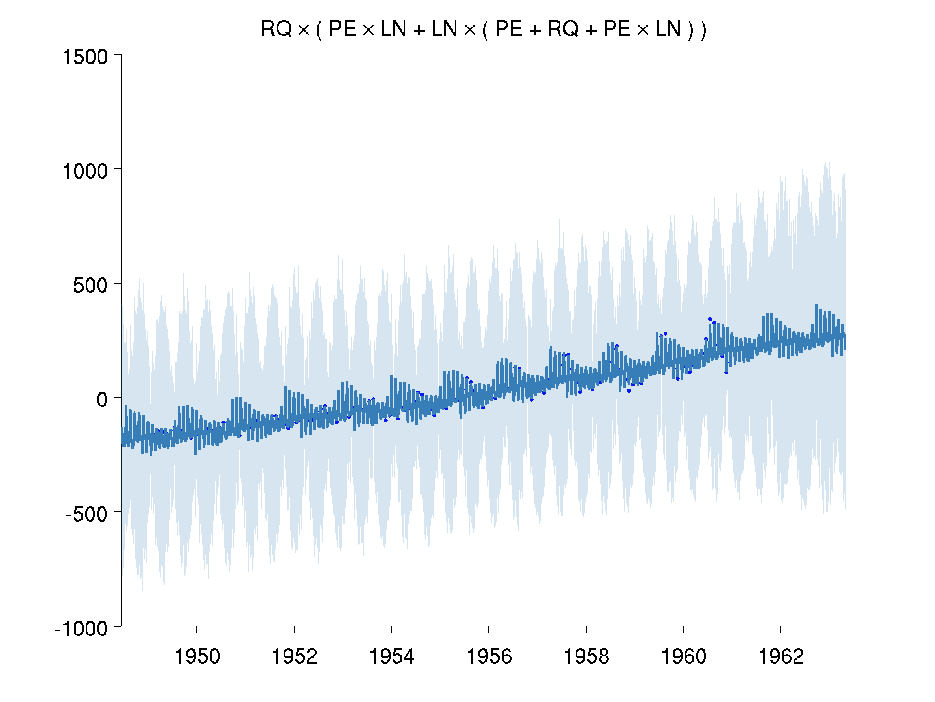
\includegraphics[width=10cm]{../figures/decomposition/01-airline/01-airline_all.pdf}
%\caption{The complete posterior on the Airline dataset.}
%\label{fig:mauna_all}
%\end{figure}

%\newcommand{\fw}{8cm}
%\begin{figure*}
%\centering
%\begin{tabular}{cc}
% 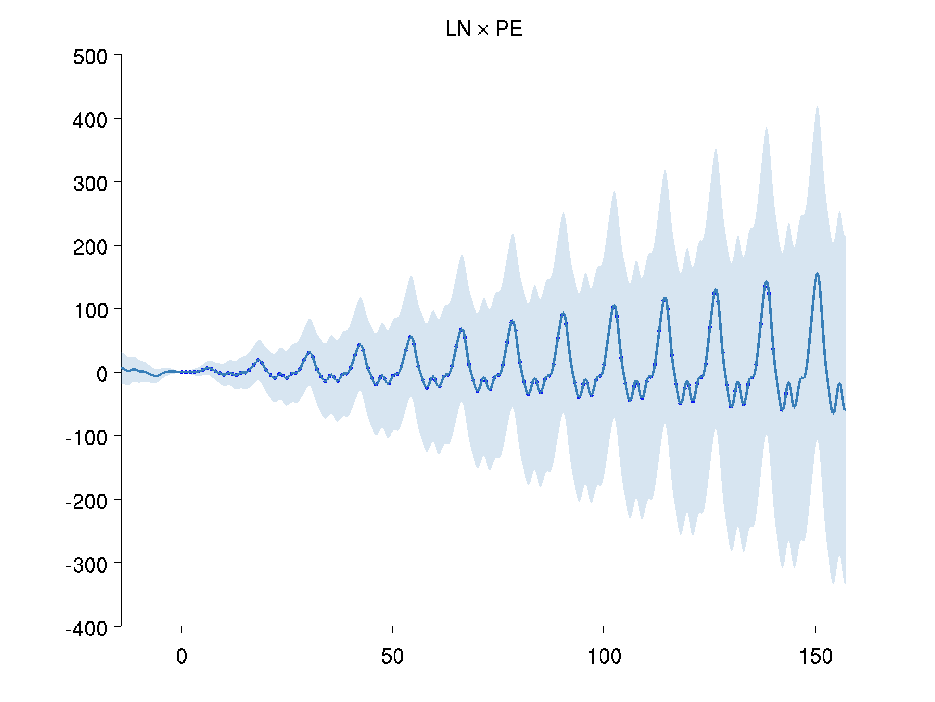
\includegraphics[width=\fw]{../figures/decomposition/01-airline/01-airline_7.pdf} &  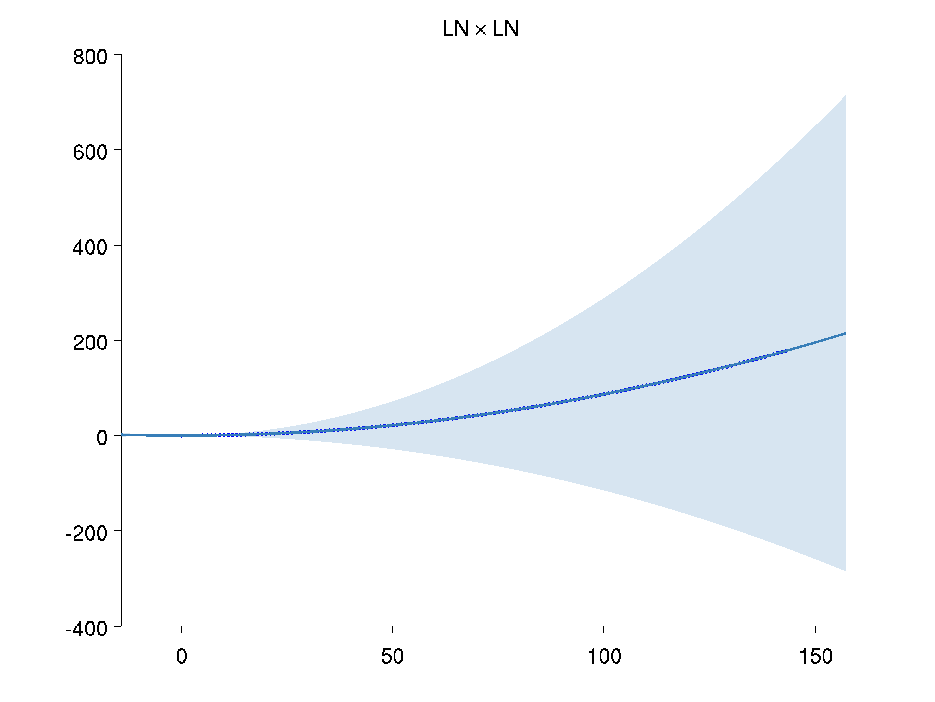
\includegraphics[width=\fw]{../figures/decomposition/01-airline/01-airline_8.pdf} \\
%  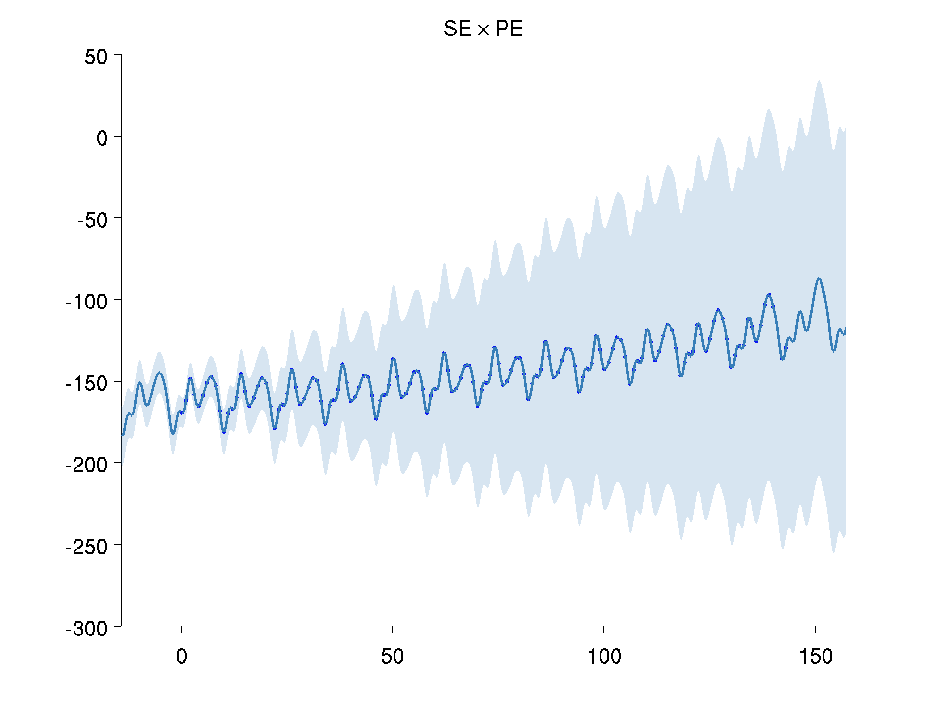
\includegraphics[width=\fw]{../figures/decomposition/01-airline/01-airline_5.pdf} &  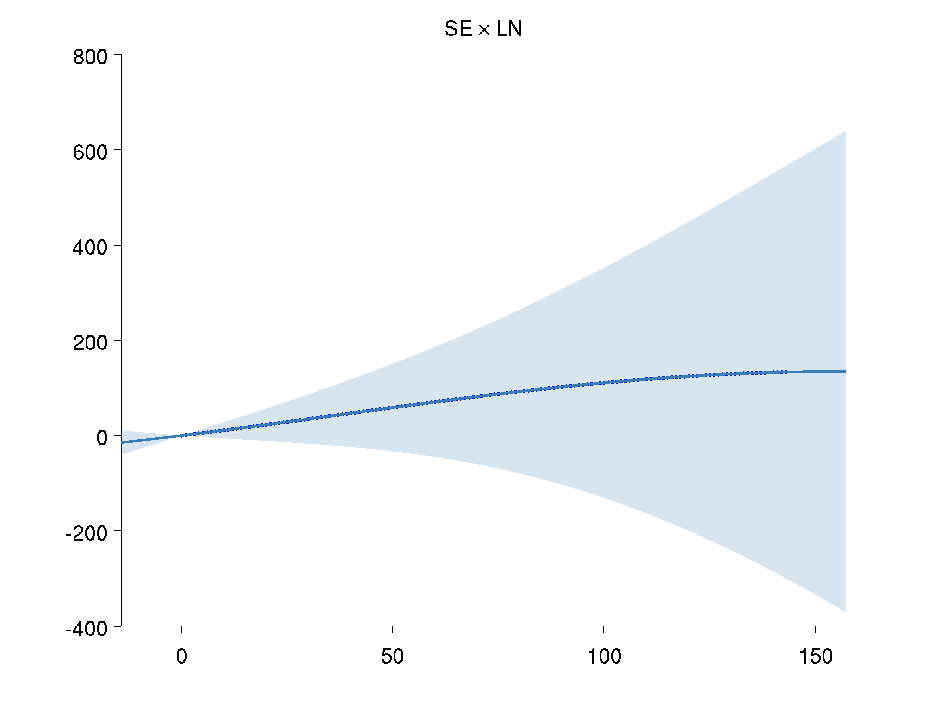
\includegraphics[width=\fw]{../figures/decomposition/01-airline/01-airline_6.pdf} \\
%   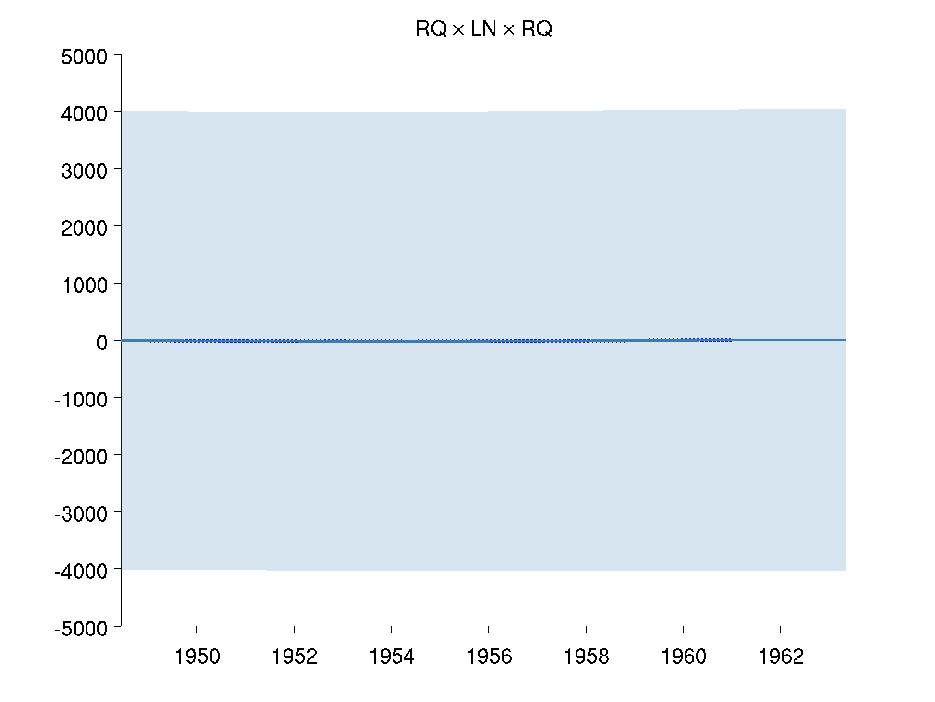
\includegraphics[width=\fw]{../figures/decomposition/01-airline/01-airline_3.pdf} &  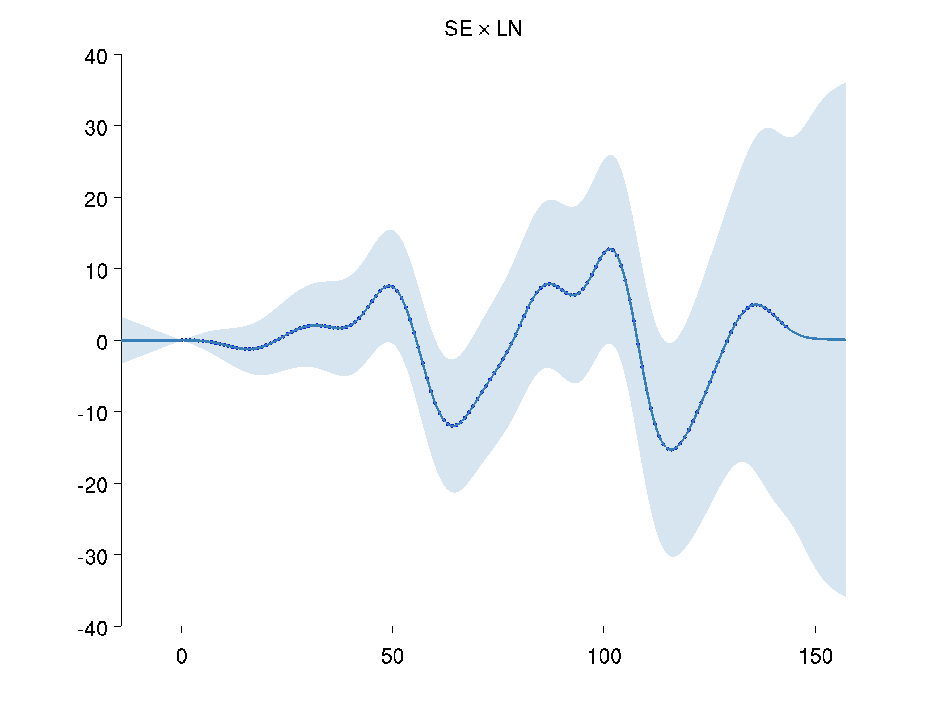
\includegraphics[width=\fw]{../figures/decomposition/01-airline/01-airline_4.pdf} \\
%    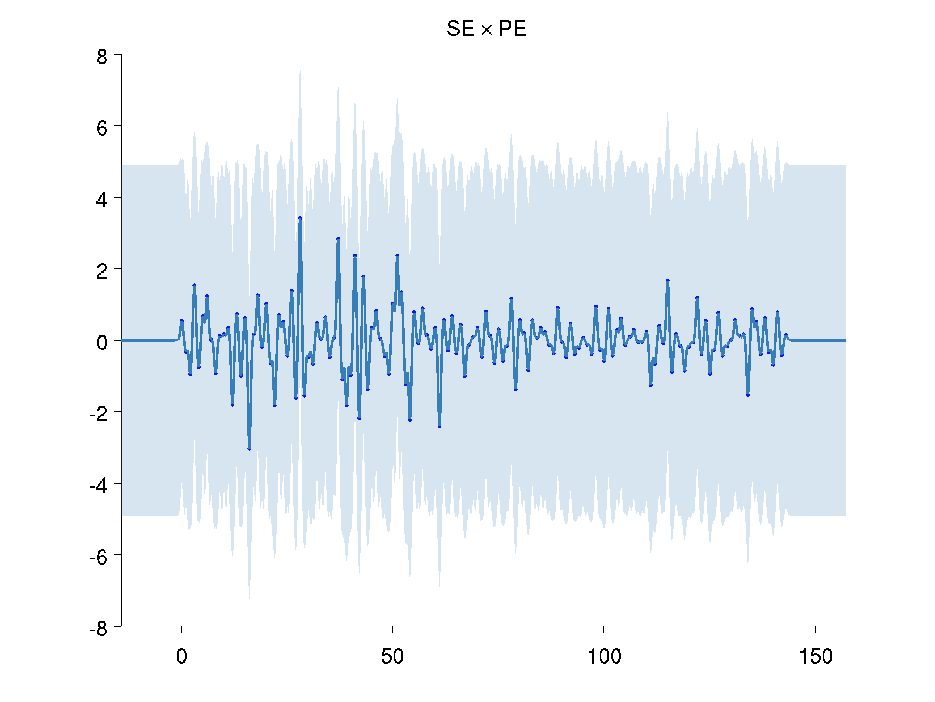
\includegraphics[width=\fw]{../figures/decomposition/01-airline/01-airline_1.pdf} &  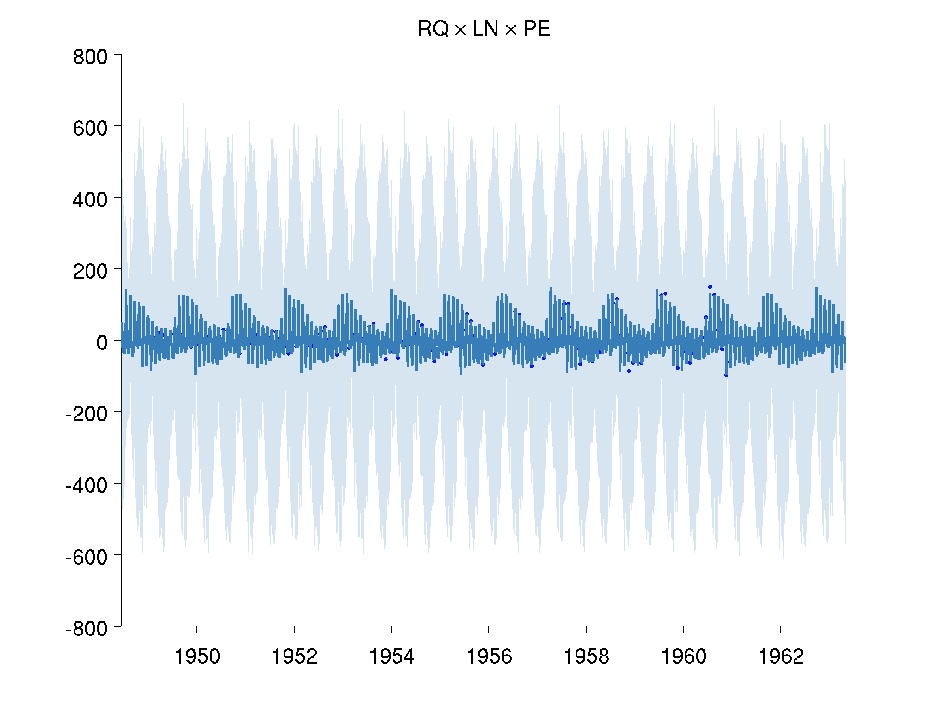
\includegraphics[width=\fw]{../figures/decomposition/01-airline/01-airline_2.pdf}
%\end{tabular}
%\caption{Automatic decomposition of airline data.
%}
%\label{fig:kernels}
%\end{figure*}


\section{Complete listings of chosen kernels}

Below, we show the best kernel structure found for each fold of the datasets used in the results tables.

%%% --- Automatically generated by latex.py ---
% Exported at 2012-11-12 20:20:44.119762
\begin{table}[h!]
\begin{center}
\begin{tabular}{l | r r r}
 Dataset  & \rotatebox{0}{ NLL }  \\ \hline
 & \rotatebox{0}{ Kernel }  \\ \hline
rconcrete & $ 348.3 $ & $ \left( M_1 \left(RQ(\ell=6.2, \alpha=-1.6, \sigma=0.2)\right) 	imes \left( M_7 \left(SE(\ell=3.5, \sigma=2.6)\right) + \left( M_0 \left(RQ(\ell=5.8, \alpha=14.5, \sigma=2.9)\right) 	imes M_3 \left(SE(\ell=3.8, \sigma=-0.1)\right) \right) \right) \right) $ & $ 348.3 $ \\
mauna & $ 166.7 $ & $ \left( M_0 \left(RQ(\ell=-1.8, \alpha=-1.3, \sigma=-1.3)\right) + M_0 \left(RQ(\ell=0.5, \alpha=-0.1, \sigma=-0.2)\right) + \left( M_0 \left(SE(\ell=4.6, \sigma=2.8)\right) 	imes M_0 \left(PE(\ell=2.0, p=-0.0, \sigma=1.7)\right) \right) \right) $ & $ 166.7 $ \\
unicyclepitchangvel & $ -656.2 $ & $ \left( M_0 \left(SE(\ell=-0.5, \sigma=0.7)\right) + \left( M_3 \left(RQ(\ell=0.5, \alpha=-0.5, \sigma=0.0)\right) 	imes M_8 \left(SE(\ell=-1.5, \sigma=-0.2)\right) 	imes M_10 \left(PE(\ell=-3.1, p=7.7, \sigma=0.6)\right) \right) \right) $ & $ -656.2 $ \\
bachsynthr & $ 20.0 $ & $ \left( M_0 \left(SE(\ell=2.4, \sigma=0.6)\right) 	imes M_1 \left(SE(\ell=2.3, \sigma=0.2)\right) 	imes M_2 \left(SE(\ell=2.4, \sigma=0.4)\right) 	imes M_3 \left(SE(\ell=2.3, \sigma=1.9)\right) \right) $ & $ 20.0 $ \\
rconcrete & $ 1598.5 $ & $ \left( M_1 \left(RQ(\ell=1.1, \alpha=-4.9, \sigma=0.2)\right) 	imes M_3 \left(RQ(\ell=-2.0, \alpha=-5.3, \sigma=-0.1)\right) 	imes \left( M_0 \left(RQ(\ell=5.5, \alpha=4.8, \sigma=3.0)\right) + M_7 \left(RQ(\ell=1.5, \alpha=-2.3, \sigma=2.5)\right) \right) \right) $ & $ 1598.5 $ \\
unicyclepitchangle & $ -1510.5 $ & $ \left( M_0 \left(RQ(\ell=0.4, \alpha=-0.1, \sigma=-1.2)\right) + \left( M_3 \left(RQ(\ell=0.9, \alpha=0.0, \sigma=-0.6)\right) 	imes M_8 \left(SE(\ell=-0.8, \sigma=0.0)\right) 	imes M_10 \left(RQ(\ell=3.8, \alpha=4.1, \sigma=-0.3)\right) \right) \right) $ & $ -1510.5 $ \\
housing & $ 1259.4 $ & $ \left( M_5 \left(SE(\ell=0.6, \sigma=2.3)\right) 	imes M_12 \left(SE(\ell=3.0, \sigma=-0.2)\right) 	imes \left( M_4 \left(RQ(\ell=-6.8, \alpha=-3.4, \sigma=0.2)\right) + M_6 \left(SE(\ell=4.2, \sigma=-0.4)\right) \right) \right) $ & $ 1259.4 $ \\
prostate & $ 110.4 $ & $ \left( \left( M_0 \left(SE(\ell=1.7, \sigma=0.7)\right) 	imes M_0 \left(PE(\ell=0.6, p=-0.0, \sigma=-0.1)\right) \right) + \left( M_1 \left(SE(\ell=0.1, \sigma=-0.4)\right) 	imes M_4 \left(SE(\ell=-1.6, \sigma=-0.1)\right) \right) \right) $ & $ 110.4 $ \\
gefload500Z & $ 128.4 $ & $ \left( M_3 \left(SE(\ell=-0.2, \sigma=0.0)\right) 	imes M_9 \left(RQ(\ell=-1.0, \alpha=-3.5, \sigma=-0.4)\right) 	imes \left( M_0 \left(PE(\ell=-0.8, p=-0.0, \sigma=-0.6)\right) + M_0 \left(RQ(\ell=-2.3, \alpha=-0.4, \sigma=0.0)\right) \right) \right) $ & $ 128.4 $ \\
pumadyn & $ 663.2 $ & $ \left( M_2 \left(SE(\ell=0.0, \sigma=1.0)\right) 	imes \left( M_1 \left(SE(\ell=0.4, \sigma=0.7)\right) + M_3 \left(SE(\ell=-0.9, \sigma=-0.6)\right) \right) \right) $ & $ 663.2 $ \\
rsolar & $  nan $ & $ M_0 \left(SE(\ell=0.0, \sigma=0.0)\right) $ & $  nan $ \\
mauna & $ 134.8 $ & $ \left( M_0 \left(SE(\ell=0.3, \sigma=-0.7)\right) + \left( M_0 \left(PE(\ell=1.2, p=-0.0, \sigma=-0.3)\right) 	imes \left( M_0 \left(RQ(\ell=-0.7, \alpha=-0.2, \sigma=-0.6)\right) + M_0 \left(RQ(\ell=4.9, \alpha=-0.7, \sigma=4.3)\right) \right) \right) \right) $ & $ 134.8 $ \\
gefload500Z & $ -421.7 $ & $ \left( M_0 \left(RQ(\ell=0.3, \alpha=-2.1, \sigma=-0.1)\right) 	imes M_9 \left(SE(\ell=1.2, \sigma=0.0)\right) 	imes \left( M_0 \left(PE(\ell=-0.8, p=0.0, \sigma=-0.9)\right) + M_0 \left(RQ(\ell=-0.5, \alpha=-2.2, \sigma=-0.1)\right) \right) \right) $ & $ -421.7 $ \\
\end{tabular}
\end{center}
\end{table}

%%% --- Automatically generated by latex.py ---
% Exported at 2013-01-21 15:40:09.878013
\begin{table*}[h!]
\begin{center}
\begin{tabular}{l | l l l}
 Dataset  & \rotatebox{0}{ NLL }  & \rotatebox{0}{ Kernel }  \\ \hline
bachsynthr200fold10of10result & $ 22.6 $ & $ CB_{0} \times QD_{1} \times P3_{2} \times QD_{3} $ \\
bachsynthr200fold1of10result & $ 163.1 $ & $ QD_{0} \times QD_{2} \times \left( SE_{0} + CB_{3} \right) $ \\
bachsynthr200fold2of10result & $ 17.5 $ & $ CB_{0} \times QD_{1} \times CB_{2} \times QD_{3} $ \\
bachsynthr200fold3of10result & $ 85.3 $ & $ MT_{0} \times QD_{3} \times \left( QD_{1} + LN_{2} \right) $ \\
bachsynthr200fold4of10result & $ 15.8 $ & $ QD_{0} \times QD_{1} \times P3_{2} \times QD_{3} $ \\
bachsynthr200fold5of10result & $ 19.2 $ & $ CB_{0} \times QD_{1} \times CB_{2} \times CB_{3} $ \\
bachsynthr200fold6of10result & $ 159.9 $ & $ QD_{0} \times QD_{2} \times \left( P3_{0} + QD_{3} \right) $ \\
bachsynthr200fold7of10result & $ 170.7 $ & $ CB_{0} \times P3_{2} \times P1_{3} $ \\
bachsynthr200fold8of10result & $ 15.7 $ & $ P3_{0} \times QD_{1} \times CB_{2} \times CB_{3} $ \\
bachsynthr200fold9of10result & $ 164.3 $ & $ QD_{0} \times CB_{2} \times \left( LN_{3} + QD_{7} \right) $ \\
rconcrete500fold10of10result & $ 191.1 $ & $ MT_{1} \times RQ_{3} \times \left( RQ_{0} + P3_{7} \right) $ \\
rconcrete500fold1of10result & $ 174.6 $ & $ RQ_{1} \times RQ_{3} \times \left( RQ_{0} + MT_{7} \right) $ \\
rconcrete500fold2of10result & $ 200.2 $ & $ MT_{1} \times \left( MT_{7} + MT_{0} \times RQ_{3} \right) $ \\
rconcrete500fold3of10result & $ 203.9 $ & $ P0_{1} \times RQ_{3} \times \left( MT_{0} + MT_{7} \right) $ \\
rconcrete500fold4of10result & $ 203.0 $ & $ P0_{1} \times RQ_{3} \times \left( P0_{0} + MT_{7} \right) $ \\
rconcrete500fold5of10result & $ 284.9 $ & $ RQ_{0} \times \left( MT_{3} + MT_{7} \right) $ \\
rconcrete500fold6of10result & $ 199.3 $ & $ MT_{1} \times RQ_{3} \times \left( MT_{0} + MT_{7} \right) $ \\
rconcrete500fold7of10result & $ 268.8 $ & $ \left( MT_{7} + MT_{0} \times RQ_{3} \right) $ \\
rconcrete500fold8of10result & $ 187.5 $ & $ MT_{0} \times P0_{1} \times RQ_{3} \times P0_{7} $ \\
rconcrete500fold9of10result & $ 188.1 $ & $ RQ_{1} \times RQ_{3} \times \left( MT_{0} + MT_{7} \right) $ \\
rhousingfold10of10result & $ 130.8 $ & $ P2_{5} \times P3_{12} \times \left( RQ_{4} + LN_{6} \right) $ \\
rhousingfold1of10result & $ 135.1 $ & $ RQ_{4} \times SE_{5} \times P2_{6} \times P2_{12} $ \\
rhousingfold2of10result & $ 145.3 $ & $ SE_{5} \times P2_{12} \times \left( RQ_{4} + LN_{6} \right) $ \\
rhousingfold3of10result & $ 151.7 $ & $ RQ_{4} \times P2_{5} \times CB_{8} \times P1_{12} $ \\
rhousingfold4of10result & $ 138.2 $ & $ SE_{5} \times P2_{12} \times \left( RQ_{4} + LN_{6} \right) $ \\
rhousingfold5of10result & $ 128.7 $ & $ QD_{5} \times P1_{12} \times \left( RQ_{4} + LN_{6} \right) $ \\
rhousingfold6of10result & $ 132.5 $ & $ SE_{5} \times P1_{12} \times \left( RQ_{4} + LN_{6} \right) $ \\
rhousingfold7of10result & $  nan $ & $ CB_{3} $ \\
rhousingfold8of10result & $ 125.5 $ & $ CB_{5} \times P1_{12} \times \left( RQ_{4} + LN_{6} \right) $ \\
rhousingfold9of10result & $ 120.5 $ & $ SE_{5} \times P1_{12} \times \left( RQ_{4} + LN_{6} \right) $ \\
rpumadyn512fold10of10result & $ 397.6 $ & $ P3_{1} \times P1_{2} $ \\
rpumadyn512fold1of10result & $ 390.6 $ & $ SE_{1} \times P2_{2} $ \\
rpumadyn512fold2of10result & $ 383.2 $ & $ SE_{1} \times \left( PE_{0} + SE_{2} \right) $ \\
rpumadyn512fold3of10result & $ 404.5 $ & $ P3_{1} \times P1_{2} $ \\
rpumadyn512fold4of10result & $ 387.1 $ & $ P3_{1} \times P3_{2} $ \\
rpumadyn512fold5of10result & $ 394.3 $ & $ P3_{1} \times P3_{2} $ \\
rpumadyn512fold6of10result & $ 402.2 $ & $ P3_{1} \times P1_{2} $ \\
rpumadyn512fold7of10result & $ 396.8 $ & $ P3_{1} \times P1_{2} $ \\
rpumadyn512fold8of10result & $ 397.7 $ & $ P3_{1} \times P1_{2} $ \\
rpumadyn512fold9of10result & $ 399.2 $ & $ P3_{1} \times P1_{2} $ \\
rservofold10of10result & $ 80.3 $ & $ MT_{0} \times CB_{1} \times CB_{2} $ \\
rservofold1of10result & $ 62.8 $ & $ P0_{0} \times CB_{2} \times \left( CB_{1} + P3_{3} \right) $ \\
rservofold2of10result & $ 53.7 $ & $ MT_{0} \times CB_{2} \times \left( CB_{1} + P3_{3} \right) $ \\
rservofold3of10result & $ 41.8 $ & $ MT_{0} \times CB_{2} \times \left( CB_{1} + SE_{3} \right) $ \\
rservofold4of10result & $ 59.6 $ & $ MT_{0} \times CB_{2} \times \left( CB_{1} + P1_{3} \right) $ \\
rservofold5of10result & $ 59.9 $ & $ MT_{0} \times CB_{2} \times \left( CB_{1} + P3_{3} \right) $ \\
rservofold6of10result & $ 56.9 $ & $ MT_{0} \times CB_{2} \times \left( CB_{1} + P3_{3} \right) $ \\
rservofold7of10result & $ 68.3 $ & $ MT_{0} \times QD_{1} \times CB_{2} $ \\
rservofold8of10result & $ 38.0 $ & $ MT_{0} \times CB_{2} \times \left( CB_{1} + P3_{3} \right) $ \\
rservofold9of10result & $ 75.6 $ & $ MT_{0} \times QD_{1} \times CB_{2} $ \\
\end{tabular}
\end{center}
\end{table*}

%%% --- Automatically generated by latex.py ---
% Exported at 2013-01-22 11:35:10.959759
\begin{table*}[h!]
\begin{center}
\begin{tabular}{l | l l l}
 Dataset  & \rotatebox{0}{ NLL }  & \rotatebox{0}{ Kernel }  \\ \hline
bachsynthr200fold10of10result & $ 24.9 $ & $ SE_{1} \times SE_{2} \times SE_{3} \times \left( SE_{0} + SE_{7} \right) $ \\
bachsynthr200fold1of10result & $ 19.0 $ & $ SE_{0} \times SE_{1} \times SE_{2} \times SE_{3} $ \\
bachsynthr200fold4of10result & $ 18.2 $ & $ SE_{0} \times SE_{1} \times SE_{2} \times SE_{3} $ \\
bachsynthr200fold5of10result & $ 22.4 $ & $ SE_{0} \times SE_{1} \times SE_{2} \times SE_{3} $ \\
bachsynthr200fold6of10result & $ 19.8 $ & $ SE_{1} \times SE_{2} \times \left( SE_{0} + SE_{5} \right) \times \left( SE_{3} + SE_{4} \right) $ \\
bachsynthr200fold7of10result & $ 21.0 $ & $ SE_{0} \times SE_{1} \times SE_{3} \times \left( SE_{2} + SE_{6} \right) $ \\
bachsynthr200fold8of10result & $ 17.9 $ & $ \left( SE_{7} + SE_{0} \times SE_{1} \times SE_{2} \times SE_{3} \right) $ \\
rconcrete500fold10of10result & $ 114.3 $ & $ SE_{0} \times SE_{6} \times \left( SE_{1} + SE_{3} \times SE_{4} \right) \times \left( SE_{3} + SE_{5} + SE_{7} \right) $ \\
rconcrete500fold1of10result & $ 125.3 $ & $ SE_{1} \times SE_{6} \times \left( SE_{0} + SE_{1} + SE_{4} \right) \times \left( SE_{3} + SE_{5} + SE_{7} \right) $ \\
rconcrete500fold2of10result & $ 154.0 $ & $ \left( SE_{0} + SE_{1} \right) \times \left( SE_{1} + SE_{3} + SE_{7} + SE_{3} \times \left( SE_{4} + SE_{5} \right) \right) $ \\
rconcrete500fold6of10result & $ 134.3 $ & $ \left( SE_{0} + SE_{3} \times SE_{4} \right) \times \left( SE_{1} + SE_{6} \right) \times \left( SE_{3} + SE_{5} + SE_{7} \right) $ \\
rconcrete500fold7of10result & $ 118.1 $ & $ \left( SE_{0} + SE_{6} \right) \times \left( SE_{1} + SE_{3} \times SE_{4} \right) \times \left( SE_{3} + SE_{5} + SE_{7} \right) $ \\
rconcrete500fold9of10result & $ 120.9 $ & $ \left( SE_{0} + SE_{6} \right) \times \left( SE_{1} + SE_{4} \right) \times \left( SE_{3} + SE_{5} + SE_{7} \right) $ \\
rhousingfold10of10result & $ 110.8 $ & $ SE_{5} \times SE_{9} \times SE_{12} \times \left( SE_{4} + SE_{6} \times SE_{11} \times SE_{12} \right) $ \\
rhousingfold2of10result & $ 104.7 $ & $ SE_{0} \times SE_{5} \times \left( SE_{4} + SE_{6} \times SE_{11} \times SE_{12} \times \left( SE_{7} + SE_{9} \right) \right) $ \\
rhousingfold4of10result & $ 107.3 $ & $ SE_{5} \times SE_{9} \times SE_{12} \times \left( SE_{4} + SE_{6} \times SE_{12} \right) \times \left( SE_{4} + SE_{11} \right) $ \\
rhousingfold8of10result & $ 95.1 $ & $ SE_{5} \times \left( SE_{4} + SE_{6} \times SE_{9} \times SE_{12} \right) \times \left( SE_{4} + SE_{11} \right) $ \\
rhousingfold9of10result & $ 89.9 $ & $ SE_{5} \times SE_{9} \times SE_{12} \times \left( SE_{4} + SE_{6} \times SE_{12} \right) \times \left( SE_{4} + SE_{11} \right) $ \\
rpumadyn512fold3of10result & $ 405.2 $ & $ SE_{1} \times SE_{2} $ \\
rpumadyn512fold4of10result & $ 387.2 $ & $ SE_{1} \times SE_{2} $ \\
rpumadyn512fold7of10result & $ 397.4 $ & $ SE_{1} \times SE_{2} $ \\
rpumadyn512fold9of10result & $ 399.8 $ & $ SE_{1} \times SE_{2} $ \\
rservofold10of10result & $ 76.3 $ & $ SE_{2} \times \left( SE_{0} + SE_{3} \right) \times \left( SE_{1} + SE_{3} \right) $ \\
rservofold3of10result & $ 60.8 $ & $ SE_{1} \times SE_{2} \times \left( SE_{3} + SE_{0} \times SE_{1} \right) $ \\
rservofold4of10result & $ 75.2 $ & $ SE_{2} \times \left( SE_{0} + SE_{3} \right) \times \left( SE_{1} + SE_{3} \right) $ \\
rservofold7of10result & $ 62.7 $ & $ SE_{1} \times SE_{2} \times \left( SE_{0} + SE_{3} \right) $ \\
\end{tabular}
\end{center}
\end{table*}

%% --- Automatically generated by latex.py ---
% Exported at 2013-01-28 10:34:20.566777
\begin{table*}[h!]
\begin{center}
\begin{tabular}{l | l l l}
 Dataset  & \rotatebox{0}{ NLL }  & \rotatebox{0}{ Kernel }  \\ \hline
bachsynthr200fold10of10result & $ 24.9 $ & $ SE_{0} \times SE_{1} \times SE_{2} \times SE_{3} $ \\
bachsynthr200fold1of10result & $ 19.0 $ & $ SE_{0} \times SE_{1} \times SE_{2} \times SE_{3} $ \\
bachsynthr200fold2of10result & $ 21.0 $ & $ SE_{0} \times SE_{1} \times SE_{2} \times SE_{3} $ \\
bachsynthr200fold3of10result & $ 21.1 $ & $ SE_{0} \times SE_{1} \times SE_{2} \times SE_{3} $ \\
bachsynthr200fold4of10result & $ 18.2 $ & $ SE_{0} \times SE_{1} \times SE_{2} \times SE_{3} $ \\
bachsynthr200fold5of10result & $ 22.4 $ & $ SE_{0} \times SE_{1} \times SE_{2} \times SE_{3} $ \\
bachsynthr200fold6of10result & $ 20.2 $ & $ SE_{0} \times SE_{1} \times SE_{2} \times SE_{3} $ \\
bachsynthr200fold7of10result & $ 21.0 $ & $ SE_{0} \times SE_{1} \times SE_{2} \times SE_{3} $ \\
bachsynthr200fold8of10result & $ 17.9 $ & $ SE_{0} \times SE_{1} \times SE_{2} \times SE_{3} $ \\
bachsynthr200fold9of10result & $ 22.2 $ & $ SE_{0} \times SE_{1} \times SE_{2} \times SE_{3} $ \\
rconcrete500fold10of10result & $ 103.8 $ & $ RQ_{1} \times RQ_{4} \times SE_{6} \times RQ_{7} \times \left( SE_{7} + RQ_{5} \times \left( RQ_{0} + SE_{3} \right) \right) $ \\
rconcrete500fold1of10result & $ 76.2 $ & $ RQ_{1} \times RQ_{4} \times SE_{6} \times RQ_{7} \times \left( RQ_{0} \times RQ_{3} + SE_{6} \times SE_{7} \right) $ \\
rconcrete500fold2of10result & $ 114.8 $ & $ SE_{1} \times RQ_{4} \times RQ_{6} \times \left( SE_{0} \times RQ_{3} + RQ_{5} \times SE_{7} \right) $ \\
rconcrete500fold3of10result & $ 111.7 $ & $ RQ_{1} \times SE_{6} \times \left( RQ_{4} + RQ_{6} \right) \times \left( RQ_{7} + RQ_{0} \times \left( RQ_{3} + SE_{7} \right) \right) $ \\
rconcrete500fold4of10result & $ 123.9 $ & $ SE_{1} \times RQ_{4} \times SE_{6} \times RQ_{7} \times \left( SE_{7} + SE_{0} \times RQ_{3} \right) $ \\
rconcrete500fold5of10result & $ 100.0 $ & $ SE_{1} \times RQ_{4} \times RQ_{5} \times SE_{6} \times RQ_{7} \times \left( SE_{7} + RQ_{0} \times RQ_{3} \right) $ \\
rconcrete500fold6of10result & $ 114.9 $ & $ SE_{0} \times SE_{1} \times RQ_{4} \times RQ_{6} \times \left( SE_{7} + SE_{3} \times SE_{5} \right) $ \\
rconcrete500fold7of10result & $ 112.9 $ & $ SE_{1} \times RQ_{4} \times RQ_{6} \times RQ_{7} \times \left( SE_{7} + RQ_{0} \times RQ_{3} \right) $ \\
rconcrete500fold8of10result & $ 89.4 $ & $ SE_{0} \times RQ_{1} \times RQ_{3} \times RQ_{4} \times RQ_{6} \times \left( RQ_{7} + RQ_{0} \times SE_{5} \right) $ \\
rconcrete500fold9of10result & $ 100.7 $ & $ SE_{0} \times SE_{1} \times RQ_{4} \times RQ_{6} \times \left( RQ_{7} + RQ_{0} \times RQ_{3} \right) $ \\
rhousingfold10of10result & $ 103.0 $ & $ RQ_{4} \times SE_{5} \times SE_{6} \times SE_{9} \times RQ_{11} \times SE_{12} $ \\
rhousingfold1of10result & $ 106.2 $ & $ SE_{0} \times RQ_{4} \times SE_{5} \times SE_{6} \times SE_{9} \times SE_{11} \times SE_{12} $ \\
rhousingfold2of10result & $ 106.8 $ & $ RQ_{4} \times SE_{5} \times SE_{6} \times SE_{9} \times SE_{12} \times \left( SE_{0} + SE_{11} \right) $ \\
rhousingfold3of10result & $ 117.6 $ & $ RQ_{4} \times SE_{5} \times SE_{6} \times SE_{9} \times SE_{12} \times \left( SE_{0} + SE_{11} \right) $ \\
rhousingfold4of10result & $ 103.5 $ & $ SE_{0} \times RQ_{4} \times SE_{5} \times SE_{6} \times SE_{11} \times SE_{12} \times \left( SE_{4} + SE_{9} \right) $ \\
rhousingfold5of10result & $ 96.8 $ & $ SE_{0} \times RQ_{4} \times SE_{5} \times SE_{6} \times SE_{9} \times SE_{11} \times SE_{12} $ \\
rhousingfold6of10result & $ 102.6 $ & $ SE_{0} \times RQ_{4} \times SE_{5} \times SE_{6} \times SE_{9} \times RQ_{11} \times SE_{12} $ \\
rhousingfold7of10result & $ 113.7 $ & $ SE_{0} \times SE_{5} \times SE_{9} \times SE_{11} \times SE_{12} \times \left( RQ_{4} + SE_{6} \right) $ \\
rhousingfold8of10result & $ 96.8 $ & $ RQ_{4} \times SE_{5} \times SE_{6} \times SE_{9} \times SE_{11} \times SE_{12} $ \\
rhousingfold9of10result & $ 88.1 $ & $ RQ_{4} \times SE_{5} \times SE_{6} \times SE_{9} \times SE_{12} \times \left( SE_{0} + SE_{11} \right) $ \\
rpumadyn512fold10of10result & $ 397.8 $ & $ SE_{1} \times SE_{2} $ \\
rpumadyn512fold1of10result & $ 390.8 $ & $ SE_{1} \times SE_{2} $ \\
rpumadyn512fold2of10result & $ 392.9 $ & $ SE_{1} \times SE_{2} $ \\
rpumadyn512fold3of10result & $ 405.2 $ & $ SE_{1} \times SE_{2} $ \\
rpumadyn512fold4of10result & $ 387.2 $ & $ SE_{1} \times SE_{2} $ \\
rpumadyn512fold5of10result & $ 394.4 $ & $ SE_{1} \times SE_{2} $ \\
rpumadyn512fold6of10result & $ 402.6 $ & $ SE_{1} \times SE_{2} $ \\
rpumadyn512fold7of10result & $ 397.4 $ & $ SE_{1} \times SE_{2} $ \\
rpumadyn512fold8of10result & $ 399.1 $ & $ SE_{1} \times SE_{2} $ \\
rpumadyn512fold9of10result & $ 393.5 $ & $ SE_{2} \times \left( SE_{1} + SE_{3} \right) $ \\
rservofold10of10result & $ 76.2 $ & $ SE_{2} \times \left( SE_{0} + SE_{3} \right) \times \left( SE_{1} + SE_{3} \right) $ \\
rservofold1of10result & $ 78.8 $ & $ RQ_{1} \times SE_{2} \times \left( SE_{0} + SE_{3} \right) $ \\
rservofold2of10result & $ 72.4 $ & $ SE_{2} \times \left( SE_{0} + SE_{3} \right) \times \left( SE_{1} + SE_{3} \right) $ \\
rservofold3of10result & $ 60.8 $ & $ RQ_{1} \times SE_{2} \times \left( SE_{0} + SE_{3} \right) $ \\
rservofold4of10result & $ 77.4 $ & $ RQ_{1} \times SE_{2} \times \left( SE_{0} + SE_{3} \right) $ \\
rservofold5of10result & $ 74.0 $ & $ SE_{2} \times \left( SE_{0} + SE_{3} \right) \times \left( SE_{1} + SE_{3} \right) $ \\
rservofold6of10result & $ 75.4 $ & $ SE_{2} \times \left( SE_{0} + SE_{3} \right) \times \left( SE_{1} + SE_{3} \right) $ \\
rservofold7of10result & $ 62.7 $ & $ SE_{1} \times SE_{2} \times \left( SE_{0} + SE_{3} \right) $ \\
rservofold8of10result & $ 65.0 $ & $ SE_{1} \times SE_{2} \times \left( SE_{0} + SE_{3} \right) $ \\
rservofold9of10result & $ 72.5 $ & $ SE_{0} \times SE_{2} \times SE_{3} \times \left( SE_{0} + SE_{1} \right) $ \\
\end{tabular}
\end{center}
\end{table*}

%% --- Automatically generated by latex.py ---
% Exported at 2013-01-29 09:18:46.732854
\begin{table*}[h!]
\begin{center}
\begin{tabular}{l | l l l}
 Dataset  & \rotatebox{0}{ NLL }  & \rotatebox{0}{ Kernel }  \\ \hline
bachsynthr200fold10of10result & $  6.0 $ & $ \left( LN_{0} + SE_{1} \right) \times \left( LN_{1} + LN_{2} + P1_{2} \right) \times \left( LN_{3} + P1_{3} \right) $ \\
bachsynthr200fold1of10result & $ -2.6 $ & $ RQ_{0} \times SE_{1} \times SE_{2} \times \left( LN_{0} + LN_{3} + LN_{1} \times LN_{2} \right) $ \\
bachsynthr200fold2of10result & $  6.1 $ & $ SE_{0} \times \left( LN_{0} + LN_{2} + LN_{3} \right) \times \left( SE_{1} + LN_{2} \right) $ \\
bachsynthr200fold3of10result & $ -1.0 $ & $ \left( SE_{0} + LN_{1} + LN_{2} + LN_{3} \right) \times \left( LN_{0} + LN_{2} + LN_{3} \right) $ \\
bachsynthr200fold4of10result & $ -10.4 $ & $ SE_{3} \times \left( LN_{0} + LN_{1} + LN_{3} \right) \times \left( LN_{0} + P1_{1} + LN_{2} \right) $ \\
bachsynthr200fold5of10result & $  6.6 $ & $ SE_{0} \times \left( LN_{0} + LN_{2} + LN_{3} \right) \times \left( SE_{1} + LN_{3} \right) $ \\
bachsynthr200fold6of10result & $ -1.1 $ & $ SE_{0} \times P1_{1} \times SE_{2} \times \left( LN_{0} + LN_{3} + LN_{1} \times LN_{2} \right) $ \\
bachsynthr200fold7of10result & $  3.8 $ & $ SE_{1} \times \left( SE_{0} + LN_{3} \right) \times \left( LN_{0} + LN_{2} + LN_{3} \right) $ \\
bachsynthr200fold8of10result & $ -3.9 $ & $ P1_{0} \times P1_{1} \times SE_{2} \times \left( LN_{0} + LN_{3} + LN_{1} \times LN_{2} \right) $ \\
bachsynthr200fold9of10result & $  5.6 $ & $ SE_{1} \times \left( SE_{0} + LN_{3} \right) \times \left( LN_{0} + LN_{2} + LN_{3} \right) $ \\
rconcrete500fold10of10result & $ 103.5 $ & $ RQ_{0} \times MT_{3} \times MT_{6} \times \left( LN_{1} + MT_{4} \right) \times \left( MT_{3} + MT_{7} \right) $ \\
rconcrete500fold1of10result & $ 93.3 $ & $ MT_{1} \times RQ_{4} \times MT_{6} \times \left( SE_{0} + P1_{6} \right) \times \left( MT_{7} + MT_{0} \times RQ_{3} \right) $ \\
rconcrete500fold2of10result & $ 114.9 $ & $ MT_{4} \times MT_{6} \times \left( MT_{1} + MT_{4} \right) \times \left( RQ_{0} \times RQ_{3} + RQ_{5} \times MT_{7} \right) $ \\
\end{tabular}
\end{center}
\end{table}


\bibliographystyle{format/icml2013}
\bibliography{gpss}

\end{document}


% Extra stuff



\section{James' Derivation of the Posterior Marginal Conditional Variance}
\begin{lem}
\label{lem:cond}
If
\begin{eqnarray}
x & \dist & \Normal(\mu, \Lambda^{-1}) \\
y \given x & \dist & \Normal(Ax + b, L^{-1})
\end{eqnarray}
then
\begin{eqnarray}
y & \dist & \Normal(A\mu + b, L^{-1} + A\Lambda^{-1}A') \\
x \given y & \dist & \Normal(\Sigma(A'L(y-b) + \Lambda\mu, \Sigma)
\end{eqnarray}
where
\begin{equation}
\Sigma = (\Lambda + A'LA)^{-1}.
\end{equation}
\end{lem}
\begin{prop}
If
\begin{eqnarray}
f_1 & \dist & \Normal(0, K_1) \\
f \given f_1 & \dist & \Normal(f_1, K_2) \\
f_1^* \given f_1 & \dist & \Normal(k_1^*K_1^{-1}f_1, K_1^{**} - k_1^*K_1^{-1}k_1^{*t})
\end{eqnarray}
then
\begin{eqnarray}
f_1 \given f & \dist & \Normal(\Sigma K_2^{-1}f, \Sigma) \\
f_1^* \given f & \dist & \Normal(k_1^*\Lambda f, K_1^{**} - k_1^*\Delta k_1^{*t})
\end{eqnarray}
where
\begin{eqnarray}
\Sigma & = & (K_1^{-1} + K_2^{-1})^{-1} \\
\Lambda & = & (K_1 + K_2)^{-1} \\
\Delta & = & K_1^{-1} - (K_1 + K_1K_2^{-1}K_1)^{-1}
\end{eqnarray}
\end{prop}

\begin{proof}
We first apply the second half of lemma~\ref{lem:cond} with $x=f_1$, $y=f$, $\mu=b=0$, $A=I$, $\Lambda^{-1} = K_1$ and $L^{-1} = K_2$ yielding
\begin{eqnarray}
f_1 \given f & \dist & \Normal(\Sigma K_2^{-1}f, \Sigma).
\end{eqnarray}
Since $f_1^*$ is independent of $f$ given $f_1$ we have $p(f_1^* \given f) = \int p(f_1^* \given f_1) p(f_1 \given f) \textrm{d}f_1$\PROBLEM{I think this is true - think graphical models} i.e.~we condition $f_1^*$ on the posterior of $f_1$.
We apply the first half of lemma~\ref{lem:cond} with $x=(f_1\given f)$, $y=f_1^*$, $\mu=\Sigma K_2^{-1}f$, $b=0$, $A = k_1^*K_1^{-1}$, $\Lambda^{-1}=\Sigma$ and $L^{-1} = K_1^{**} - k_1^*K_1^{-1}k_1^{*t}$.
Then for the mean of $f_1^* \given f$ we get the expression
\begin{eqnarray}
& k_1^*K_1^{-1} \Sigma K_2^{-1}f \\
= & k_1^*K_1^{-1} (K_1^{-1} + K_2^{-1})^{-1} K_2^{-1}f \\
= & k_1^*(K_1 + K_2)^{-1}f \\
= & k_1^*\Lambda f
\end{eqnarray}
and for the variance we obtain
\begin{eqnarray}
& K_1^{**} - k_1^*K_1^{-1}k_1^{*t} + k_1^*K_1^{-1} \Sigma K_1^{-1}k_1^{*t} \\
= & K_1^{**} - k_1^*(K_1^{-1} - (K_1 + K_1K_2^{-1}K_1)^{-1})k_1^{*t} \\
= & K_1^{**} - k_1^*\Delta k_1^{*t}
\end{eqnarray}
\end{proof}






\section{Load forecasting}

Similar to the above, we apply the methodology to another highly structured time series, but with additional input data.
We analyse hourly load data for a US utility; this data was recently the focus of a data mining competition; the load forecasting track of GEFCom2012\footnotemark.
The data consists of hourly load measurements of a US utility over several years, split into 20 geographical zones and 11 temperature time series.
The relationships (geographical or otherwise) between the zones and the temperature stations were unknown for the purposes of the competition.

\footnotetext{\texttt{http://www.gefcom.org/}}
\begin{figure}
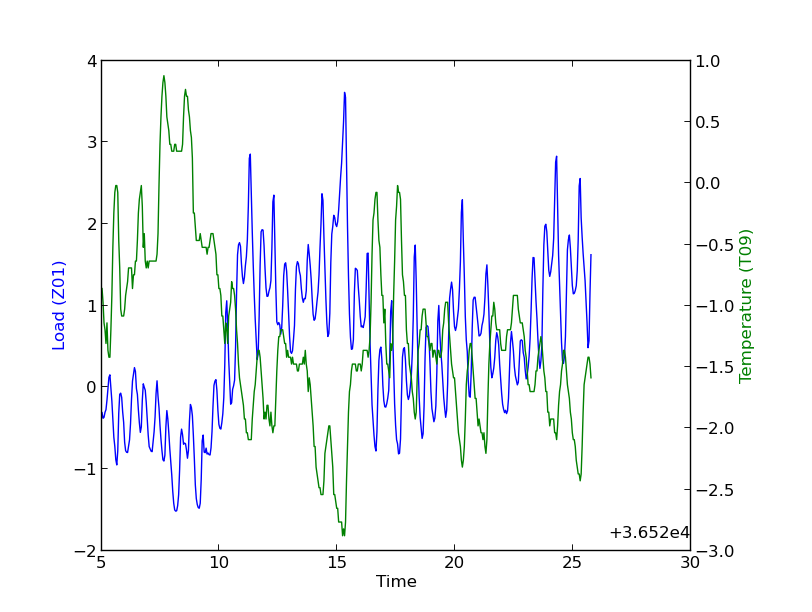
\includegraphics[width=0.5\columnwidth]{../figures/gef_load_z01_t09_500}
\caption{Zone 1 and temperature station 9 from GEFCom2012 load forecasting data.}
\label{fig:gef_z01_t09}
\end{figure}

Figure~\ref{fig:gef_z01_t09} shows the first 500 data points (approx.~20 days) of zone 1 together with temperature station 9 (all data has been standardised to have zero mean and unit standard deviation).
The plot shows that the load data follows a smooth trend with near periodic deviations.
The overall trend is somehow related to the temperature and some of the spikes in the load data appear to be related to spikes in temperature.

We applied our kernel selection methodology to this data set (using all temperature stations).
The kernels discovered at subsequent levels of the search were:
\begin{enumerate}
\item \texttt{RQ\_t(-1.8,  0.0, -1.0)}
\item \texttt{RQ\_t(-1.4,  0.0, -2.1) + PE\_t(-0.7,  0.0, -0.8)}
\item \texttt{RQ\_t( 0.3, -0.1, -1.9) * ( PE\_t(-0.9,  0.0, -1.0) + RQ\_t(-0.6,  0.0, -2.2) )}
\item \texttt{RQ\_t( 0.3, -0.1, -2.1) * SE\_T9( 1.2,  0.0) * ( PE\_t(-0.8,  0.0, -0.9) + RQ\_t(-0.5, -0.1, -2.2) )}
\end{enumerate}
The learnt kernels can be interpreted as follows.
The simplest model explains the data as a smooth function of time, with a short lengthscale to account for all of the variation.
The next model explains the data as a sum of a smooth component and periodic component with a period of one day; the lengthscale of the smooth component has increased since some of the fine detail can be explained by the periodic component.
The next model also splits the function into smooth and periodic components, but the periodic component is multiplied by a rational quadratic kernel which allows it to vary smoothly through time; again the lengthscale of the smooth component has increased since the fine detail has been better explained by the periodic component.
Finally, the model introduces a temperature variable to further explain the observed data.

One can visualise how the different components of the kernel capture the structure of the data.
Figure~\ref{fig:gef_z01_two_means} shows the components of the Gaussian process posterior mean corresponding to the additive components of the kernel function (after expanding brackets and grouping product terms).

\begin{figure}
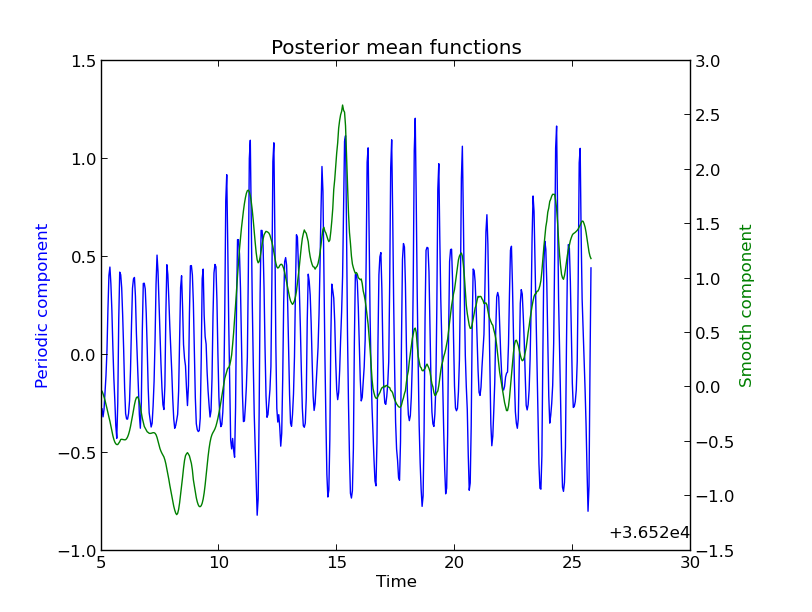
\includegraphics[width=0.5\columnwidth]{../figures/gef_load_z01_500_posteriors}
\caption{Zone 1 from GEFCom 2012 separated into smooth and periodic component}
\label{fig:gef_z01_two_means}
\end{figure}

\TBD{Not sure the below is going to work.}
These posterior means have been evaluated at a particular 1 dimensional trace through time and temperature.
We can however examine the posterior mean of the Gaussian process at other points in time and temperature space to better understand the interaction.
\TBD{If we plot the smooth component, it would be super awesome if we could see the weekend or other interpretable blips in time, whilst most of the variation in the trend might be explained by temperature. Kernel might not be complicated enough to really show this though \frownie.}

\TBD{What else can we say about this data? Numerical results might take a while to produce.}


